\section{Programming using packet transactions}
\label{s:transactions}
\begin{figure*}[!t]
\begin{minipage}{0.6\textwidth}
\begin{small}
\begin{lstlisting}[style=customc]
#define NUM_FLOWLETS    8000
#define THRESHOLD       5
#define NUM_HOPS        10

struct Packet {
  int sport;
  int dport;
  int new_hop;
  int arrival;
  int next_hop;
  int id; // array index
};

int last_time [NUM_FLOWLETS] = {0};
int saved_hop [NUM_FLOWLETS] = {0};

void flowlet(struct Packet pkt) {
  pkt.new_hop = hash3(pkt.sport,
                      pkt.dport,
                      pkt.arrival)
                % NUM_HOPS;

  pkt.id  = hash2(pkt.sport,
                  pkt.dport)
            % NUM_FLOWLETS;

  if (pkt.arrival - last_time[pkt.id] 
      > THRESHOLD) 
  { saved_hop[pkt.id] = pkt.new_hop; }

  last_time[pkt.id] = pkt.arrival;
  pkt.next_hop = saved_hop[pkt.id];
}
\end{lstlisting}
\end{small}
\end{minipage}
%
\vrule\quad
%
\begin{minipage}{0.4\textwidth}
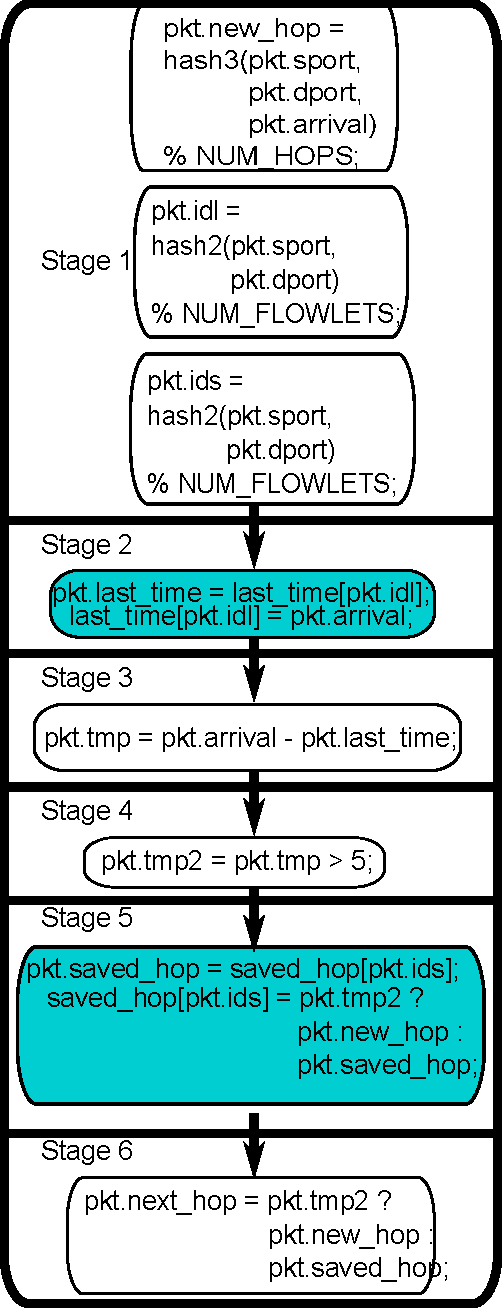
\includegraphics[width=0.8\columnwidth]{pipe.pdf}
\end{minipage}
\caption{\small (a) Flowlet switching written \pktlanguage (left);
(b) Compiled 6-stage pipeline in \absmachine implementing (a).  Control flows
from top to bottom. Atoms manipulating state are shaded in blue (right).}
\label{fig:flowlet}
\end{figure*}


We now illustrate programming using packet transactions in \pktlanguage, using
flowlet switching~\cite{flowlets} as an example. Flowlet switching is a
load-balancing algorithm that sends bursts of packets (called flowlets) from a
TCP flow on different paths, provided the bursts are separated by a large
enough interval in time to ensure that packets do not arrive out of order at
the TCP receiver. Figure~\ref{fig:flowlet} shows how flowlet switching is
expressed in \pktlanguage. For simplicity, the example hashes only the source
and destination ports of a packet; it is easy to extend this to hash the full
5-tuple.

This example demonstrates the core language constructs in \pktlanguage. All
packet processing happens in the context of a packet transaction (the function
\texttt{flowlet} on line 17), a C function that takes a C struct as an
argument. The struct declares the fields in a packet (lines 5--12)\footnote{We
  use fields to refer to both packet headers such as source port (sport) and
destination port (dport) and packet metadata (id).} that can be referenced by the
function body (lines 18--32).  In addition, the function body can reference
state variables that represent persistent state stored on the switch. These are
declared as global variables at the program top level (e.g. \texttt{last\_time}
and \texttt{saved\_hop} on lines 14 and 15).

Conceptually, the packet transaction function modifies its packet argument in
place until the end of the function body, before processing the next packet.
\pktlanguage forbids return statements implying that execution will always end at the
end of the function body. The function body may also call out to intrinsic
functions such as \texttt{hash2} on lines 23 and \texttt{hash3} on line 18.
These represent hardware primitives provided by the abstract machine that
aren't interpreted by \pktlanguage. The \pktlanguage compiler uses the
signature of intrinsic functions to infer dependencies and supplies a canned
run-time implementation for these functions, but otherwise doesn't interpret or
analyze their implementation. Finally, the packet
transaction's body is written in a constrained subset of C that excludes all
iterative constructs. The function body can include if and else-if statements,
but all other control transfer (break, goto, switch, return, and continue
statements) is forbidden.

\pktlanguage forbids pointers and dynamic memory allocation. Arrays can be used
as state variables, but with restrictions. While a packet transaction's body is
being executed for a specific packet, all accesses to an array variable must use the
same index. For subsequent packets, this index can be different. For instance,
all accesses to the arrays \texttt{last\_time} and \texttt{saved\_hop} use the
index \texttt{pkt.id} that is constant for each packet, but changes from one
packet to the next. This restriction simplifies the treatment of arrays in the
compiler, while still allowing us to express several data-plane algorithms of
practical interest.

These restrictions seem severe at first glance, but are required to provide
deterministic performance guarantees. Memory allocation, unbounded iteration
counts for loops, and unrestricted control transfer all cause variable run-time
performance.

When compiled to an instance of the \absmachine abstract machine (\S\ref{s:absmachine}), the
\pktlanguage compiler converts the code in Figure~\ref{fig:flowlet}a into the
pipelined form shown in Figure~\ref{fig:flowlet}b. Today, programmable switch
chips are programmed by manually specifying low-level pipeline configurations
resembling Figure~\ref{fig:flowlet}b using a language like P4 or an API such as
Cavium's XPliant SDK~\cite{xpliant_sdk} or Intel's Ethernet
SDK~\cite{intel_sdk}. This is a difficult and error-prone
process~\cite{p4-semantics}.  Programming in \pktlanguage lets a compiler
automate this process: the user doesn't worry about hardware details such as
pipeline stages and concurrency within each stage.
